\chapter{Managing Partitions}

\section{Understanding Disk Layout}
There are two basic ways of organizing data on a hard disk : Partitions and LVM (Logical Volume Management). Some parts of a hard disk need to be configured with a fixed amount of storage. In such cases we use partitions. This is applicable for \verb|/boot| and \verb|/| in the figure. However, certain directories contain dynamic user data, and thus need to be able to grow to any size. In such cases, the partitions don't work and we need to use Logical Volumes. In the image below, \verb|sda1, sda2 & sda3| are all Physical Volume(PV)s or partitions. In linux, each partition needs to be connected to one or more directories in order to be used. 

\begin{figure}[H]
	\centering
	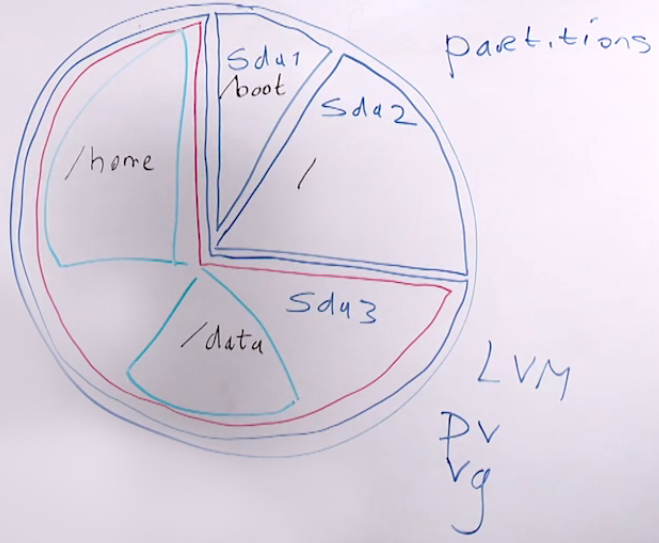
\includegraphics[width=0.9\linewidth]{RHCSA/Mod2/chapters/2.15.a}
	\caption{Disk Layout}
	\label{fig:2 Disk Layout}
\end{figure}


In the case of Logical Volumes (LVs), just like partitions, there needs to be a Physical Volume (PV). This PV is then put in a Volume Group (Vg), represented by the red boundary lines in the image above. From this volume group, we can create Logical Volumes (represented by the blue lines). The advantage of this method is the unused space between different LVs can be added to any of the LVs, and thus no disk space is wasted and no directory in the LV is going to be full while another is barely filled. In LVM it's very easy to grow a logical volume later!

	\section{Creating Partitions}
To add a new disk to our OS, first we need to verify the storage disks that are available. For this we use the \textbf{proc} filesystem in \verb|/proc/|. It acts as an interface to everything that's happening in the kernel. The \verb|/proc/partitions| file contains a listing of all the disks and partitions that are currently existing.

\vspace{-15pt}
\begin{minted}{console}
$ cat /proc/partitions
major minor  #blocks  name

8        0   20971520 sda
8        1       2048 sda1
8        2     499712 sda2
8        3   15634432 sda3
8       16   10485760 sdb
11        0    8491008 sr0
253        0    3903488 dm-0
253        1    1953792 dm-1
253        2    1953792 dm-2
253        3    7815168 dm-3
\end{minted}
\vspace{-10pt}

\noindent
While \textit{sda} is the first hard disk, the device \textit{sdb} is a newly added one - the second hard disk avaiable in the computer. The partitions are marked by a number after the device name - \textit{sda1, sda2 and sda3}. The second hard disk doesn't have any partitions yet.

\subsection{fdisk}
\textbf{fdisk} is an old partitioning tool that has been revised for RHEL 7. Running the \verb|fdisk| utility on \verb|/dev/sdb|, the location which the OS uses to designate the second hard disk yeilds:

\vspace{-15pt}
\begin{minted}{console}
# fdisk /dev/sdb
Welcome to fdisk (util-linux 2.23.2).

Changes will remain in memory only, until you decide to write them.
Be careful before using the write command.

Device does not contain a recognized partition table
Building a new DOS disklabel with disk identifier 0xf11ab429.

Command (m for help): 
\end{minted}
\vspace{-10pt}

\noindent
It tells us that the disk doesn't contain any partitions (since it's brand new). The fdisk utility offers us a bunch of commands, among which we'll use:

\noindent
\begin{tabular}{lM{0.84}}
	\toprule
	\textbf{Options} &\textbf{Description} \\
	\midrule
	\textbf{p}	&Print partition table \\
	\textbf{n}	&Add a new partition \\
	\textbf{w}	&Write the table to disk and exit \\
	\bottomrule
\end{tabular}

\subsubsection{p command}
\vspace{-10pt}
The p option gives us the current disk layout:

\vspace{-15pt}
\begin{minted}{bash}
Command (m for help): p

Disk /dev/sdb: 10.7 GB, 10737418240 bytes, 20971520 sectors
Units = sectors of 1 * 512 = 512 bytes
Sector size (logical/physical): 512 bytes / 512 bytes
I/O size (minimum/optimal): 512 bytes / 512 bytes
Disk label type: dos
Disk identifier: 0xf11ab429

Device Boot      Start         End      Blocks   Id  System

Command (m for help): 
\end{minted}
\vspace{-10pt}

\noindent
The device name is \textit{sdb} and its size is 10.7GB. This gives it 20 Million sectors, since the size of each sector is 512B. Now we add a new partition on the disk:

\vspace{-15pt}
\begin{minted}{bash}
Command (m for help): n
Partition type:
p   primary (0 primary, 0 extended, 4 free)
e   extended
Select (default p): p
Partition number (1-4, default 1): 
First sector (2048-20971519, default 2048): 
Using default value 2048
Last sector, +sectors or +size{K,M,G} (2048-20971519, default 20971519): +100M
Partition 1 of type Linux and of size 100 MiB is set

Command (m for help): 
\end{minted}
\vspace{-10pt}

\noindent
The default option at the prompt can be selected by simply pressing the enter key. Since there are no physical partitions already available, and since we should always choose the option to add physical partitions whenever possible, we add a new physical partition. It asks us for the starting sector, the default of which is 2048. The first 2MBs are used to store metadata. Next, we mark the end of the partition using a relative size: in this case, of 100MiB ($1024^2$B). The size has to be specified with uppercase K/M/G to not be misconstrued to any other unit. Printing the partition table now shows:

\vspace{-15pt}
\begin{minted}{bash}	
Device Boot         Start         End      Blocks   Id  System
/dev/sdb1            2048      206847      102400   83  Linux
\end{minted}
\vspace{-10pt}

\noindent
This new partition can then be written to the disk using \verb|w|. 

\vspace{-15pt}
\begin{minted}{bash}
Command (m for help): w
The partition table has been altered!

Calling ioctl() to re-read partition table.
Syncing disks.
\end{minted}
\vspace{-10pt}

\noindent
Now when we view the partitions in \verb|/proc/partitions| we see:

\vspace{-15pt}
\begin{minted}{console}
# cat /proc/partitions
major minor  #blocks  name

8        0   20971520 sda
8        1       2048 sda1
8        2     499712 sda2
8        3   15634432 sda3
8       16   10485760 sdb
8       17     102400 sdb1
11        0    8491008 sr0
253        0    3903488 dm-0
253        1    1953792 dm-1
253        2    1953792 dm-2
253        3    7815168 dm-3
\end{minted}
\vspace{-10pt}

\noindent
The disk now has a sdb1 partition of size 100MiB. This indicates that the disk is now ready to accept a filesystem. In case an error is show along the lines of "\textit{the device is busy}", the system probably needs a restart. 

\section{Understanding File System Differences}
For a RHEL 7 installation, there are several file system choices:

\noindent
\begin{tabular}{lM{0.84}}
	\toprule
	\textbf{File System} &\textbf{Description} \\
	\midrule
	\textbf{XFS}	&The default file system for RHEL 7 and many others, built with scalability in mind. Based on a B-Tree database, which specializes in disk space allocation with high speed and makes looking up files really easy. It also has different tuning options for varying workloads. \\
	\midrule
	\textbf{Ext4}	&This was the default filesystem till RHEL 6. It was based on 1993's Ext2 file system which was built to handle much smaller disks than our current needs. It uses H-Tree indexing, which is use of basic index files - suitable for thousands of files, but not practical or economical (in terms of time) for millions of files, which our systems demand. While it is not as scalable as XFS, it does provide backwards compatibility. Thus, for best performance, it shouldn't be used as a default file system. \\
	\midrule
	\textbf{Btrfs}	&This is a Copy-on-Write(CoW) file system, which means that before writing to a file, that file is copied somewhere else, thus making journaling unnecessary! Journalling is the system where the filesystem keeps track of the changes being made to the file to make rolling back possible. This also makes undelete operations unnecessary (which have never worked on Linux anyway). It even has added features like subvolumes. It wasn't however included in RHEL 7 First Customer Shipment (FCS). \\
	\midrule
	\textbf{vfat}	&Primarily for compatibility with other OSs, such as Windows. It is particularly useful for removable media such as USB sticks. This filesystem is not needed to be installed on the hard disk of the server however, even in cases where Samba provides access to files on the server (Samba handles the file system differences and translation itself). \\
	\midrule
	\textbf{GFS2}	&For Active/Active High Availability (HA) Clustering Environments. Only needed when multiple nodes need to write to the same file system concurrently. For Active/Passive File HA Clusters, XFS/Ext4/etc. suffice. \\
	\midrule
	\textbf{Gluster}	&Gluster is a distributed file system. Thus, even though represented under the same hierarchy, it can reside on multiple servers. Storage is configured to be done in \textit{bricks} that are spread over servers. Each brick uses XFS as their back-end file system. This is an important file system for cloud environments. \\
	\bottomrule
\end{tabular}

\section{Making the File System}
Just after being created, a partition contains no file system, and thus no files can yet be stored on it. We have to create an appropriate file system using:

\subsection{mkfs}
This is actually a whole bunch of different utilities that are grouped together under the same command. They are:

\vspace{-15pt}
\begin{minted}{bash}
mkfs         mkfs.btrfs   mkfs.cramfs  mkfs.ext2    mkfs.ext3    mkfs.ext4    mkfs.fat     mkfs.minix   mkfs.msdos   mkfs.vfat    mkfs.xfs     
\end{minted}
\vspace{-10pt}

\noindent
Since the default file system is \verb|XFS|, \verb|mkfs.xfs| is the default file system utility. 

\vspace{-15pt}
\begin{minted}{console}
# mkfs.xfs --help
mkfs.xfs: invalid option -- '-'
unknown option -- 
Usage: mkfs.xfs
/* blocksize */		[-b log=n|size=num]
/* metadata */		[-m crc=0|1,finobt=0|1,uuid=xxx]
/* data subvol */	[-d agcount=n,agsize=n,file,name=xxx,size=num,
(sunit=value,swidth=value|su=num,sw=num|noalign),
sectlog=n|sectsize=num
/* force overwrite */	[-f]
/* inode size */	[-i log=n|perblock=n|size=num,maxpct=n,attr=0|1|2,
projid32bit=0|1]
/* no discard */	[-K]
/* log subvol */	[-l agnum=n,internal,size=num,logdev=xxx,version=n
sunit=value|su=num,sectlog=n|sectsize=num,
lazy-count=0|1]
/* label */		[-L label (maximum 12 characters)]
/* naming */		[-n log=n|size=num,version=2|ci,ftype=0|1]
/* no-op info only */	[-N]
/* prototype file */	[-p fname]
/* quiet */		[-q]
/* realtime subvol */	[-r extsize=num,size=num,rtdev=xxx]
/* sectorsize */	[-s log=n|size=num]
/* version */		[-V]
devicename
<devicename> is required unless -d name=xxx is given.
<num> is xxx (bytes), xxxs (sectors), xxxb (fs blocks), xxxk (xxx KiB),
xxxm (xxx MiB), xxxg (xxx GiB), xxxt (xxx TiB) or xxxp (xxx PiB).
<value> is xxx (512 byte blocks).
\end{minted}
\vspace{-10pt}

\noindent
The \textbf{block size (-b)} should be larger when primarily dealing with large files. This way, lesser blocks are used, and the administration of large files becomes easier. The \textbf{inode size (-i)} should be larger if it is known beforehand that lots of advanced stuff that stores metadata in inodes will be used. The \textit{label (-L)} sets the name for that filesystem. To actually create the file system, we use the command:

\vspace{-15pt}
\begin{minted}{console}
meta-data=/dev/sdb1              isize=512    agcount=4, agsize=65536 blks
         =                       sectsz=512   attr=2, projid32bit=1
         =                       crc=1        finobt=0, sparse=0
data     =                       bsize=4096   blocks=262144, imaxpct=25
         =                       sunit=0      swidth=0 blks
naming   =version 2              bsize=4096   ascii-ci=0 ftype=1
log      =internal log           bsize=4096   blocks=2560, version=2
         =                       sectsz=512   sunit=0 blks, lazy-count=1
realtime =none                   extsz=4096   blocks=0, rtextents=0
\end{minted}
\vspace{-10pt}

	\section{Mounting the Partition Manually}
The new partition is mounted using the \verb|mount| command. For recurring mounting, it's advisable to create a permanent mounting directory. For temporary mounts, we can use \verb|/mnt|. The mounting operation can be verified by typing the \verb|mount| command. The command to mount the new partition \verb|sdb1| on the \verb|/mnt| directory is :

\vspace{-15pt}
\begin{minted}{console}
# mount /dev/sdb1 /mnt
# mount | tail -n 5
tmpfs on /run/user/1000 type tmpfs (rw,nosuid,nodev,relatime,seclabel,size=592968k,mode=700,uid=1000,gid=1000)
fusectl on /sys/fs/fuse/connections type fusectl (rw,relatime)
gvfsd-fuse on /run/user/1000/gvfs type fuse.gvfsd-fuse (rw,nosuid,nodev,relatime,user_id=1000,group_id=1000)
/dev/sr0 on /run/media/somu/CentOS 7 x86_64 type iso9660 (ro,nosuid,nodev,relatime,uid=1000,gid=1000,iocharset=utf8,mode=0400,dmode=0500,uhelper=udisks2)
/dev/sdb1 on /mnt type xfs (rw,relatime,seclabel,attr2,inode64,noquota)
\end{minted}
\vspace{-10pt}

\noindent
\textbf{Mounting} means connecting some device or functionality to a particular directory. This not only includes removable media and peripheral device directories, but also many system settings (such as the \verb|/proc| file system or the \verb|/sys| file system). 

To view only the devices that have been mounted, we can use:

\vspace{-15pt}
\begin{minted}{console}
# mount | grep ^/dev
/dev/mapper/centos-root on / type xfs (rw,relatime,seclabel,attr2,inode64,noquota)
/dev/mapper/centos-home on /home type xfs (rw,relatime,seclabel,attr2,inode64,noquota)
/dev/sda2 on /boot type xfs (rw,relatime,seclabel,attr2,inode64,noquota)
/dev/mapper/centos-var on /var type xfs (rw,relatime,seclabel,attr2,inode64,noquota)
/dev/sr0 on /run/media/somu/CentOS 7 x86_64 type iso9660 (ro,nosuid,nodev,relatime,uid=1000,gid=1000,iocharset=utf8,mode=0400,dmode=0500,uhelper=udisks2)
/dev/sdb1 on /mnt type xfs (rw,relatime,seclabel,attr2,inode64,noquota)
\end{minted}
\vspace{-10pt}

\subsection{umount}
The \verb|umount| command is used to unmount a mounted directory. This is to ensure that no files are open and cannot be damaged by the sudden removal of the file system. The \verb|umount| command takes as parameter either the device name or the directory where it is mounted. So, both \verb|/dev/sdb1| and \verb|/mnt| are valid parameters to unmount the new partition. 

\vspace{-15pt}
\begin{minted}{console}
# umount /dev/sdb1
# mount | grep ^/dev
/dev/mapper/centos-root on / type xfs (rw,relatime,seclabel,attr2,inode64,noquota)
/dev/mapper/centos-home on /home type xfs (rw,relatime,seclabel,attr2,inode64,noquota)
/dev/sda2 on /boot type xfs (rw,relatime,seclabel,attr2,inode64,noquota)
/dev/mapper/centos-var on /var type xfs (rw,relatime,seclabel,attr2,inode64,noquota)
/dev/sr0 on /run/media/somu/CentOS 7 x86_64 type iso9660 (ro,nosuid,nodev,relatime,uid=1000,gid=1000,iocharset=utf8,mode=0400,dmode=0500,uhelper=udisks2)
\end{minted}
\vspace{-10pt}

\noindent
The device \verb|/dev/sdb1| is no longer mounted, as can be seen from the output. A major challenge that may be presented by this is the fact that the device names may change at any time! Today the device that's called \verb|/dev/sdb1| may change to \verb|/dev/sdc1| if the OS detects the devices (and names them) in another order, thus making our references to them useless. For this reason the \textit{Universally Unique ID (UUID)} of a device can be used to refer to it. The UUID of all existing devices can be displayed using:

\vspace{-15pt}
\begin{minted}{console}
# blkid
/dev/sda2: UUID="1c55e935-8099-49c4-8c72-0bc1ff7c396a" TYPE="xfs" 
/dev/sda3: UUID="DfepDW-igyh-eI6D-SgBB-3HV5-QTQT-EI3Pc2" TYPE="LVM2_member" 
/dev/sdb1: LABEL="myfs" UUID="00a8c244-8781-492c-a6ad-85624780e1e8" TYPE="xfs" 
/dev/sr0: UUID="2017-09-06-10-53-42-00" LABEL="CentOS 7 x86_64" TYPE="iso9660" PTTYPE="dos" 
/dev/mapper/centos-root: UUID="d2fe3168-4eef-431b-9a8e-eb59dae10bcb" TYPE="xfs" 
/dev/mapper/centos-swap: UUID="24b0103c-d574-4623-bc85-9255076e3b7d" TYPE="swap" 
/dev/mapper/centos-var: UUID="ed13b5f3-1b26-48f7-81cb-03a2bad5fc61" TYPE="xfs" 
/dev/mapper/centos-home: UUID="710a33e6-7e52-4c06-830d-e53ae0d58fed" TYPE="xfs" 
\end{minted}
\vspace{-10pt}

\noindent
As can be seen, the label for the file system is also shown using the \verb|blkid| command. Both the UUID and the label for the file system can be used to reference the device while using the mount command:

\vspace{-15pt}
\begin{minted}{console}
# mount LABEL=myfs /mnt
# mount | tail -n 3
gvfsd-fuse on /run/user/1000/gvfs type fuse.gvfsd-fuse (rw,nosuid,nodev,relatime,user_id=1000,group_id=1000)
/dev/sr0 on /run/media/somu/CentOS 7 x86_64 type iso9660 (ro,nosuid,nodev,relatime,uid=1000,gid=1000,iocharset=utf8,mode=0400,dmode=0500,uhelper=udisks2)
/dev/sdb1 on /mnt type xfs (rw,relatime,seclabel,attr2,inode64,noquota)
\end{minted}
\vspace{-10pt}

	\section{Understanding /etc/fstab}
The names of the devices in \verb|/etc/fstab| are not based on their actual device names, but either the LVM volume names or their UUID. The typical \verb|/etc/fstab| file looks like:

\vspace{-15pt}
\begin{minted}{bash}
# cat fstab

#
# /etc/fstab
# Created by anaconda on Sat Nov 25 08:44:04 2017
#
# Accessible filesystems, by reference, are maintained under '/dev/disk'
# See man pages fstab(5), findfs(8), mount(8) and/or blkid(8) for more info
#
/dev/mapper/centos-root /                       xfs     defaults        0 0
UUID=1c55e935-8099-49c4-8c72-0bc1ff7c396a /boot                   xfs     defaults        0 0
/dev/mapper/centos-home /home                   xfs     defaults        0 0
/dev/mapper/centos-var  /var                    xfs     defaults        0 0
/dev/mapper/centos-swap swap                    swap    defaults        0 0
\end{minted}
\vspace{-10pt}

\noindent
The first parameter is the UUID or the LVM volume name. The second is the directory in the FHS where the disk will be mounted. This is followed by the file system type and then the mount options. The first among the last two numbers is the option for backup support, specifically an old utility called dump-backup. Some enterprise backup utilities need dump functionality provided by this option to operate, even though they don't really use the dump-backup program. The last number is \verb|fsck| - file system check. The concept is to check the file system at boot time before it is mounted and data on it is accessed. There are three valid options: \textbf{0} (off), \textbf{1} (check the root [\verb|/|] file system) and finally \textbf{2} (check non-root file system). 

	\section{Mounting partitions via /etc/fstab}
To automount the device \verb|/dev/sdb1|, all we need to do is add the following line to \verb|/etc/fstab|:

\vspace{-15pt}
\begin{minted}{bash}
/dev/sdb1	/data	xfs		defaults	1	2
\end{minted}
\vspace{-10pt}

\noindent
Note however that the above won't guarantee that the \textit{proper} file system will always be mounted as it's dependent on the order in which the OS detects the disks! So, it's better to use the UUIDs of the file systems to track them.  We use the UUID to auto mount the file system with:

\vspace{-15pt}
\begin{minted}{bash}	
#
# /etc/fstab
# Created by anaconda on Sat Nov 25 08:44:04 2017
#
# Accessible filesystems, by reference, are maintained under '/dev/disk'
# See man pages fstab(5), findfs(8), mount(8) and/or blkid(8) for more info
#
/dev/mapper/centos-root /                       xfs     defaults        0 0
UUID=1c55e935-8099-49c4-8c72-0bc1ff7c396a /boot                   xfs     defaults        0 0
/dev/mapper/centos-home /home                   xfs     defaults        0 0
/dev/mapper/centos-var  /var                    xfs     defaults        0 0
/dev/mapper/centos-swap swap                    swap    defaults        0 0
UUID=00a8c244-8781-492c-a6ad-85624780e1e8 /data xfs     defaults        1 2
\end{minted}
\vspace{-10pt}

\noindent
To confirm the mount, we use the \verb|mount -a| command, which tries to mount everything that hasn't been mounted yet.

\vspace{-15pt}
\begin{minted}{console}
# mount -a
mount: mount point /data does not exist
\end{minted}
\vspace{-10pt}

\noindent
In this case, since the directory \verb|/data| doesn't exist, the mounting failed. The mount system doesn't create a new directory (mounting location) if it doesn't yet exist. We remedy this by:

\vspace{-15pt}
\begin{minted}{console}
# ls
bin  boot  dev  downloads  etc  home  lib  lib64  media  mnt  opt  proc  root  run  sbin  srv  sys  tmp  usr  var
# mkdir data
# mount -a 
# mount | grep ^/dev/
/dev/mapper/centos-root on / type xfs (rw,relatime,seclabel,attr2,inode64,noquota)
/dev/mapper/centos-home on /home type xfs (rw,relatime,seclabel,attr2,inode64,noquota)
/dev/sda2 on /boot type xfs (rw,relatime,seclabel,attr2,inode64,noquota)
/dev/mapper/centos-var on /var type xfs (rw,relatime,seclabel,attr2,inode64,noquota)
/dev/sr0 on /run/media/somu/CentOS 7 x86_64 type iso9660 (ro,nosuid,nodev,relatime,uid=1000,gid=1000,iocharset=utf8,mode=0400,dmode=0500,uhelper=udisks2)
/dev/sdb1 on /mnt type xfs (rw,relatime,seclabel,attr2,inode64,noquota)
/dev/sdb1 on /data type xfs (rw,relatime,seclabel,attr2,inode64,noquota)
\end{minted}
\vspace{-10pt}

\noindent
As is evident from the last line of the output, the file system has been properly mounted and is ready for use. An alternative way to mount it using fstab would've been to use the label for the disk instead of the UUID, such as:

\vspace{-15pt}
\begin{minted}{bash}
LABEL=myfs	/data	xfs	defaults	1	2
\end{minted}
\vspace{-10pt}

\subsection{Managing xfs file systems using xfs\_ commands}
The new xfs file system provides a set of commands that start with \verb|xfx_| that help administer any xfs partition. They are:

\vspace{-15pt}
\begin{minted}{bash}
xfs_admin      xfs_copy       xfs_estimate   xfs_fsr        xfs_info       
xfs_logprint   xfs_metadump   xfs_ncheck     xfs_repair     xfs_bmap       
xfs_db         xfs_freeze     xfs_growfs     xfs_io         xfs_mdrestore  
xfs_mkfile     xfs_quota      xfs_rtcp       
\end{minted}
\vspace{-10pt}

\noindent
To add a new label to the boot device, we use \verb|xfs_admin| command with the \verb|-L| command. Let us say, we want to label the boot partition on our system. To find out which partition is mapped to \verb|/boot| we use the \verb|lsblk| command. 

\vspace{-15pt}
\begin{minted}{console}
# lsblk
NAME            MAJ:MIN RM  SIZE RO TYPE MOUNTPOINT
sda               8:0    0   20G  0 disk 
sda1            8:1    0    2M  0 part 
sda2            8:2    0  488M  0 part /boot
sda3            8:3    0 14.9G  0 part 
centos-root 253:0    0  3.7G  0 lvm  /
centos-swap 253:1    0  1.9G  0 lvm  [SWAP]
centos-var  253:2    0  1.9G  0 lvm  /var
centos-home 253:3    0  7.5G  0 lvm  /home
sdb               8:16   0   10G  0 disk 
sdb1            8:17   0    1G  0 part /data
sr0              11:0    1  8.1G  0 rom  /run/media/somu/CentOS 7 x86_64
# blkid
/dev/sda2: UUID="1c55e935-8099-49c4-8c72-0bc1ff7c396a" TYPE="xfs" 
/dev/sda3: UUID="DfepDW-igyh-eI6D-SgBB-3HV5-QTQT-EI3Pc2" TYPE="LVM2_member" 
/dev/sdb1: LABEL="myfs" UUID="00a8c244-8781-492c-a6ad-85624780e1e8" TYPE="xfs" 
/dev/sr0: UUID="2017-09-06-10-53-42-00" LABEL="CentOS 7 x86_64" TYPE="iso9660" PTTYPE="dos" 
/dev/mapper/centos-root: UUID="d2fe3168-4eef-431b-9a8e-eb59dae10bcb" TYPE="xfs" 
/dev/mapper/centos-swap: UUID="24b0103c-d574-4623-bc85-9255076e3b7d" TYPE="swap" 
/dev/mapper/centos-var: UUID="ed13b5f3-1b26-48f7-81cb-03a2bad5fc61" TYPE="xfs" 
/dev/mapper/centos-home: UUID="710a33e6-7e52-4c06-830d-e53ae0d58fed" TYPE="xfs" 
# xfs_admin -L bootdevice /dev/sda2
xfs_admin: /dev/sda2 contains a mounted filesystem

fatal error -- couldn't initialize XFS library
\end{minted}
\vspace{-10pt}

\noindent
The \verb|/boot| partition was auto-mounted at start up, and thus it needs to be unmounted first before it can be edited. So, we take the following steps:

\vspace{-15pt}
\begin{minted}{console}
# umount /boot
# xfs_admin -L bootdevice /dev/sda2
writing all SBs
new label = "bootdevice"
# mount -a
# blkid
/dev/sda2: LABEL="bootdevice" UUID="1c55e935-8099-49c4-8c72-0bc1ff7c396a" TYPE="xfs" 
/dev/sda3: UUID="DfepDW-igyh-eI6D-SgBB-3HV5-QTQT-EI3Pc2" TYPE="LVM2_member" 
/dev/sdb1: LABEL="myfs" UUID="00a8c244-8781-492c-a6ad-85624780e1e8" TYPE="xfs" 
/dev/sr0: UUID="2017-09-06-10-53-42-00" LABEL="CentOS 7 x86_64" TYPE="iso9660" PTTYPE="dos" 
/dev/mapper/centos-root: UUID="d2fe3168-4eef-431b-9a8e-eb59dae10bcb" TYPE="xfs" 
/dev/mapper/centos-swap: UUID="24b0103c-d574-4623-bc85-9255076e3b7d" TYPE="swap" 
/dev/mapper/centos-var: UUID="ed13b5f3-1b26-48f7-81cb-03a2bad5fc61" TYPE="xfs" 
/dev/mapper/centos-home: UUID="710a33e6-7e52-4c06-830d-e53ae0d58fed" TYPE="xfs" 
\end{minted}
\vspace{-10pt}

	\section{Understanding Encrypted Partitions}
\begin{center}
	\verb|VIDEO TUTORIAL MISSING|
\end{center}

\section{Creating a LUKS Encrypted Partition}
To create the encrypted partition, we once again use the \verb|fdisk| utility. Since we want to put this partition on the \verb|/dev/sdb| device, we use:

\vspace{-15pt}
\begin{minted}{console}
# fdisk /dev/sdb
Welcome to fdisk (util-linux 2.23.2).

Changes will remain in memory only, until you decide to write them.
Be careful before using the write command.


Command (m for help): p

Disk /dev/sdb: 10.7 GB, 10737418240 bytes, 20971520 sectors
Units = sectors of 1 * 512 = 512 bytes
Sector size (logical/physical): 512 bytes / 512 bytes
I/O size (minimum/optimal): 512 bytes / 512 bytes
Disk label type: dos
Disk identifier: 0xf11ab429

Device Boot      Start         End      Blocks   Id  System
/dev/sdb1         2048     2099199     1048576   83  Linux
\end{minted}
\vspace{-10pt}

\noindent
At first we ensure that sufficient disk space is available via printing the existing file system details on the disk. In this example, we can see that the number of available sectors on the disk is $20,971,520$ while the End=$2,099,199$ tells us that only those sectors are used till now. Thus, we can add a new encrypted partition. The initial procedure is same as creating a normal partition:

\vspace{-15pt}
\begin{minted}{console}
Command (m for help): n  
Partition type:
p   primary (1 primary, 0 extended, 3 free)
e   extended
Select (default p): p
Partition number (2-4, default 2): 
First sector (2099200-20971519, default 2099200): 
Using default value 2099200
Last sector, +sectors or +size{K,M,G} (2099200-20971519, default 20971519): +100M
Partition 2 of type Linux and of size 100 MiB is set

Command (m for help): p

Disk /dev/sdb: 10.7 GB, 10737418240 bytes, 20971520 sectors
Units = sectors of 1 * 512 = 512 bytes
Sector size (logical/physical): 512 bytes / 512 bytes
I/O size (minimum/optimal): 512 bytes / 512 bytes
Disk label type: dos
Disk identifier: 0xf11ab429

Device Boot      Start         End      Blocks   Id  System
/dev/sdb1         2048     2099199     1048576   83  Linux
/dev/sdb2      2099200     2303999      102400   83  Linux

Command (m for help): w
The partition table has been altered!

Calling ioctl() to re-read partition table.

WARNING: Re-reading the partition table failed with error 16: Device or resource busy.
The kernel still uses the old table. The new table will be used at
the next reboot or after you run partprobe(8) or kpartx(8)
Syncing disks.

# partprobe /dev/sdb
# cat /proc/partitions
major minor  #blocks  name

8        0   20971520 sda
8        1       2048 sda1
8        2     499712 sda2
8        3   15634432 sda3
8       16   10485760 sdb
8       17    1048576 sdb1
8       18     102400 sdb2
11       0    8491008 sr0
253      0    3903488 dm-0
253      1    1953792 dm-1
253      2    1953792 dm-2
253      3    7815168 dm-3	
\end{minted}
\vspace{-10pt}

\noindent
The \verb|partprobe /dev/sdb| command updates the kernel parititon table, i.e., tells the kernel about the changes in the partition table on that device so that the kernel can provide the required functionality. 

\subsection{Formatting the new partition}
To encrypt the new partition we use the \verb|cryptsetup| command. An argument of \verb|luksFormat| is required to specify the encryption formatting. We encrypt \verb|/dev/sdb2| by:

\vspace{-15pt}
\begin{minted}{console}
# cryptsetup luksFormat /dev/sdb2

WARNING!
========
This will overwrite data on /dev/sdb2 irrevocably.

Are you sure? (Type uppercase yes): YES
Enter passphrase: 
Verify passphrase: 
#
\end{minted}
\vspace{-10pt}

\noindent
Now that our encrypted partition has been created, we need to open it to use it. For this we can use a custom-made dedicated mount point such as \verb|/secret|. Then, we have to open the partition using \verb|cryptsetup luskOpen| before we can mount it. At this point, we also have to provide a name for the partition. Finally, we go to the \verb|/dev/mapper| directory to ensure that the new partition has been successfully loaded.

\vspace{-15pt}
\begin{minted}{console}
# cryptsetup luksOpen /dev/sdb2 secret
Enter passphrase for /dev/sdb2: 
[root@vmPrime /]# cd /dev/mapper
[root@vmPrime mapper]# ls 
centos-home  centos-root  centos-swap  centos-var  control  secret
\end{minted}
\vspace{-10pt}

\noindent
Since we can see the required partition in the \verb|/dev/mapper| directory, we can be sure that the partition was opened successfully! The complete path of our partition is \verb|/dev/mapper/secret|. Now we can proceed to create a file system on it: (let's assume we want to format the disk as ext4)

\vspace{-15pt}
\begin{minted}{console}
# mkfs.ext4 /dev/mapper/secret
mke2fs 1.42.9 (28-Dec-2013)
Filesystem label=
OS type: Linux
Block size=1024 (log=0)
Fragment size=1024 (log=0)
Stride=0 blocks, Stripe width=0 blocks
25168 inodes, 100352 blocks
5017 blocks (5.00%) reserved for the super user
First data block=1
Maximum filesystem blocks=33685504
13 block groups
8192 blocks per group, 8192 fragments per group
1936 inodes per group
Superblock backups stored on blocks: 
8193, 24577, 40961, 57345, 73729

Allocating group tables: done                            
Writing inode tables: done                            
Creating journal (4096 blocks): done
Writing superblocks and filesystem accounting information: done 
\end{minted}
\vspace{-10pt}

\noindent
The encrypted partition is now ready to be mounted and used. We do this by:

\vspace{-15pt}
\begin{minted}{console}
# mkdir /secret
# mount /dev/mapper/secret /secret
# cd /secret
\end{minted}
\vspace{-10pt}

\noindent
While we normally might never need to close the encrypted partition, if for example we have a partition that's stored on an external device, we first need to unmount it, followed by performing a \verb|cryptsetup luksClose|.

\vspace{-15pt}
\begin{minted}{console}
[root@vmPrime ~]# umount /secret
[root@vmPrime ~]# cryptsetup luksClose /dev/mapper/secret
[root@vmPrime ~]# ls -l /dev/mapper
total 0
lrwxrwxrwx. 1 root root       7 Dec  8 06:51 centos-home -> ../dm-3
lrwxrwxrwx. 1 root root       7 Dec  8 06:51 centos-root -> ../dm-0
lrwxrwxrwx. 1 root root       7 Dec  8 06:51 centos-swap -> ../dm-1
lrwxrwxrwx. 1 root root       7 Dec  8 06:51 centos-var -> ../dm-2
crw-------. 1 root root 10, 236 Dec  8 06:51 control
\end{minted}
\vspace{-10pt}

\noindent
The folder \verb|/secret| within \verb|/dev/mapper| has disappeared as it's been saved to the original encrypted partition where no one can access the data without decryption. 

Now, if we want to automount the partition, we need to add an entry for it in the \verb|/etc/fstab| file:

\vspace{-15pt}
\begin{minted}{bash}
/dev/mapper/secret	/secret	ext4	defaults	1 2
\end{minted}
\vspace{-10pt}

\noindent
However, the above code work since at the time the \verb|/etc/fstab| file is processes, there is no \verb|/dev/mapper/secret| directory during boot since the file system on the encrypted partition won't be open yet! To do this, we need to create/edit the \verb|/etc/crypttab| file, with the following contents:

\vspace{-15pt}
\begin{minted}{bash}
secret	/dev/sda2	none
\end{minted}
\vspace{-10pt}

\noindent
The first value in the file is the name that's to be assigned to the partition in the \verb|/dev/mapper/| directory, the second is the device name, and the third, the name of password file to be used. Since we're not using a password file, we've left it as \textit{none}. Thus, the system will prompt for the passphrase at boot to open and mount the LUKS encrypted device. Now, to confirm the auto mounting of the device, we need to reboot. 

\section{Dealing with "Enter root password for maintenance mode"}
If there is an error within our \verb|/etc/fstab| file, our OS will fail to boot. This puts us in emergency mode, which lets us log in as the root user to troubleshoot. Since it's a boot-time error, a good idea is to use the \verb|journalctl -xb| to view the \verb|journald| logs, which may help us locate the problem. 

If the error is along the line of "the device timed out", then there is probably a typo in the device name. We can then fix the error and reboot the server.